\subsection{Ein bisschen Typografie}
\begin{frame}[fragile]{Absatzauszeichnung}
  \begin{itemize}
    \item Zur Erinnerung: Leerzeile im Code erzeugt neuen Absatz
    \item Zwei Möglichkeiten: Einzug der ersten Zeile oder vertikaler Abstand
    \item Standard ist Einzug
    \item halbzeiliger vertikaler Abstand mit:
      \begin{block}{Klassenoption}
        \begin{lstlisting}
          \documentclass[parskip=half, ...]{scrartcl}
        \end{lstlisting}
      \end{block}
  \end{itemize}
\end{frame}

\begin{frame}[fragile]{\texttt{microtype}}
  \begin{itemize}
    \item Ihr werdet den Effekt kaum sehen
    \item Das ist Absicht!
    \item Kleine Korrekturen, die das Schriftbild verbessern
    \item z.\,B. - etwas in den Rand hinein für homogenen Grauanteil
      \begin{Packages}
        \begin{lstlisting}
          \usepackage{microtype}
        \end{lstlisting}
      \end{Packages}
  \end{itemize}
\end{frame}

\begin{frame}[fragile]{Schönere Brüche im Text}
  \begin{Packages}
    \begin{lstlisting}
      \usepackage{xfrac}
    \end{lstlisting}
  \end{Packages}
  \begin{itemize}
    \item Problem: \lstinline+\frac{1}{2}+ zu hoch
    \item unschöne Alternative: 1/2
    \item schön: \lstinline+\sfrac{1}{2}+
  \end{itemize}
  \begin{CodeExample}{0.5}
    \begin{lstlisting}
      \sfrac{1}{2}
      \sfrac{$\mathup{\pi}$}{2}
    \end{lstlisting}
  \CodeResult
    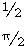
\includegraphics[scale=0.8]{figures/xfrac.pdf}
  \end{CodeExample}
\end{frame}

\begin{frame}[fragile]{Geschützte Leerzeichen}
  \begin{itemize}
    \item Es gibt Leerzeichen an denen nicht umgebrochen werden soll
    \item Zwischen Titel und Name
    \item Bei Referenzen
    \item Zweiteilige Abkürzungen (aber ein kleines!)
    \item Bei Datumsangaben
    \item Zweiteilige Ortsnamen
    \item Zwischen Zahl und Einheit (→ \texttt{siunitx})
  \end{itemize}
  \begin{CodeExample}{0.5}
    \begin{lstlisting}
      Prof.~Dr.~Dr.~Rhode
      Abbildung~\ref{fig:peplogo}
      z.\,B.
      2.~Oktober~2014
      St.~Helena
    \end{lstlisting}
    \CodeResult
      Prof.~Dr.~Dr.~Rhode \\
      Abbildung~\ref{fig:peplogo} \\
      z.\,B. \\
      2.~Oktober~2014 \\
      St.~Helena
  \end{CodeExample}
\end{frame}

\begin{frame}[fragile]{Striche}
  \begin{block}{Benötigte Einstellung}
    \begin{lstlisting}
      \defaultfontfeatures{Ligatures=TeX} % nach fontspec
    \end{lstlisting}
  \end{block}
  Es gibt vier verschiedene Striche:
  \begin{CodeExample}{0.49}
    \begin{lstlisting}
      - $-$ -- ---
    \end{lstlisting}
  \CodeResult
    - $-$ -- ---
  \end{CodeExample}

  \begin{description}[-- Halbgeviertstrich (en-dash)]
    \item[- Bindestrich]
      \begin{itemize}
        \item Bindestrich
        \item zwischen Doppelnamen der selben Person
          \begin{lstlisting}
            Levi-Civita-Symbol
          \end{lstlisting}
      \end{itemize}
    \item[-- Halbgeviertstrich (en-dash)]
      \begin{itemize}
        \item Gedankenstrich: \lstinline+ Text -- oh, Gedankenstriche -- Text +
        \item zwischen Namen von versch. Personen
          \smallskip
          \begin{lstlisting}
            Maxwell--Boltzmann-Verteilung
          \end{lstlisting}
          \smallskip
        \item ist auch der Streckenstrich
          \smallskip
          \begin{lstlisting}
            1 bis 10 ist 1--10
          \end{lstlisting}
          \smallskip
      \end{itemize}
    \item[--- Geviertstrich (em-dash)]
      \begin{itemize}
          \item nicht im Deutschen, englischer Gedankenstrich
            \begin{lstlisting}
              text---oh, em-dashes---text
            \end{lstlisting}
      \end{itemize}
  \end{description}
\end{frame}

\begin{frame}[fragile]{
  Trennung bei Strichen \hfill
  \doc{http://mirrors.ctan.org/macros/latex/contrib/ncctools/doc/extdash.pdf}{extdash}
}
  \vspace*{-2em}
  \begin{Packages}
    \begin{lstlisting}
      \usepackage[shortcuts]{extdash} % nach hyperref, bookmark
    \end{lstlisting}
  \end{Packages}

  Falls ein Wort Striche enthält, trennt \LaTeX\ ausschließlich an diesen.\\
  So ermöglicht man mehr Trennung:
  \vspace{-0.5em}
  \begin{CodeExample}{0.85}[Trennbare Striche]
    \begin{lstlisting}
      \-/ \-- \---
      Maxwell--Boltzmann-Verteilung
      Maxwell\--Boltzmann\-/Verteilung
    \end{lstlisting}
  \CodeResult
    - -- --- \\
    Maxwell--Boltzmann-Verteilung \\
    Maxwell\--Boltzmann\-/Verteilung
  \end{CodeExample}

  \vspace{-7em}
  So verhindert man die Trennung an den Strichen:
  \begin{lstlisting}
    \=/ \== \===
    $x$\=/Achse
  \end{lstlisting}
\end{frame}

\begin{frame}[fragile]{Silbentrennung}
  \begin{itemize}
    \item Manchmal kann \LaTeX\ ein Wort nicht richtig trennen
    \item Manche Fachwörter sollten nicht nach deutschen Regeln getrennt werden
  \end{itemize}
  \begin{block}{Trennung für Wort vorgeben}
    \begin{lstlisting}
      % Präambel
      \hyphenation{Dia-mag-ne-tis-mus hy-phen-ate hy-phen-a-tion}
      % statt Di-a-mag-ne-tis-mus

      hy\-phen\-ate % im Text
    \end{lstlisting}
  \end{block}
\end{frame}
